\section{Studies with the Hadron Outer Calorimeter}
	In this section some studies on detection efficiency of high energetic muons in the hadron outer calorimeter (HO) using 2012 data are shown.
	The analysis of the detection efficiency for cosmic muons from GRIN data is conclusively dealt with.
	\subsection{Studies on detection efficiency of prompt muons using 2012 data}
		Due to the similarity of the setup of HO and MTT, by studying the HO signals we expect to find answers to some open questions concerning the MTT concept e.g. the muon detection capability of a
		scintillator system read out by SiPMs e.g.
		In particular the detection efficiency for tight ID muons from Run A of the 2012 data in HO has been studied.
		The used dataset (/SingleMu/Run2012A-22Jan2013-v1/RECO) is from the re-reconstruction campain Jan 2013.
		Thereby the SingleMu stream contains several HLT trigger paths each with at least one triggered muon with different conditions like a $p_t$ requirement or an isolation criterion.
		In this note we won't go into the details of the composition of the SingleMu stream. 
		The muons from this dataset have to fulfill some selection criteria and also they have to be accepted by the HO system.
		The latter is necessary due to the inefficient areas of HO caused for example by the supporting structures of CMS like the chimney (\cite{JINST}).
		But before this selection can be done, the events have to fulfill some cleaning procedure.
		First of all the events from beam background are removed.
		Than a primary vertex filter is applied:
		Using the vertex collection \textit{offlinePrimaryVertices} only the events are chosen, in which vertices could be found whose:
			\begin{itemize}
				\item minimum number of degrees of freedom is 4,
				\item maximum distance on the $z$ axis to the origin of the coordinate system is 24\,cm,
				\item maximum impact parameter $d_0$ is 2\,cm.
			\end{itemize}
		\subsubsection{Muon selection and acceptance by HO}
		\label{thesectionhere}
			To be sure to have no fake muons going through the HO tiles some selection criteria are set for the reconstructed muons.
			First of all only reconstructed global muons are chosen.
			Their transverse momentum $p_t$ should be greater than 26\,GeV.
			Then a cut on the pseudorapidity of the muons $|\eta_\mu| < 0.9$ is applied to be ensure that they are in the barrel region and especially in the region of HO.
			Furthermore the muons also have to have a tight ID.
			In \cite{CMS-PAPER-MUO-10-004} all requirements on muons to be a tight muon are given.
			Additionally all these selected tight muons should have a particle flow based combined relative isolation $I$ defined as
			\begin{equation}
				I = \frac{\sum{E_T^{chHad}} + \sum{E_T^{neutHad}} + \sum{E_T^\gamma}}{p_T}
			\end{equation}
			where $E_T^{chHad}$ is the transverse energy of a charged hadron in a cone of $\Delta R = 0.4$ around the muon, $E_T^{neutHad}$ same for a neutral hadron and $E_T^\gamma$ for a photon.
			Since the HO system does not cover the whole $\eta$-$\phi$ plane - for example there are no tiles between the wheels - and also since the HO system has some areas with electronic inefficiencies the
			cut on $|\eta_{mu}|$ mentioned before is not sufficient and a more sophisticated geometrical acceptance have to be required.
			This is done by using the \textit{MuonHOAcceptance} class implemented in CMSSW.
			\textit{MuonHOAcceptance} contains the entire HO geometry and allows boolean decisions on whether a muon is in the geometrical acceptance of the HO or not and also whether a muon is in the
			acceptance region of tiles which are working properly.
			It is also possible to accept or reject muons in regions with SiPM instrumented tiles (figure \ref{fig:ho_acceptance}).
			\begin{figure}[htbp]
				\centering
				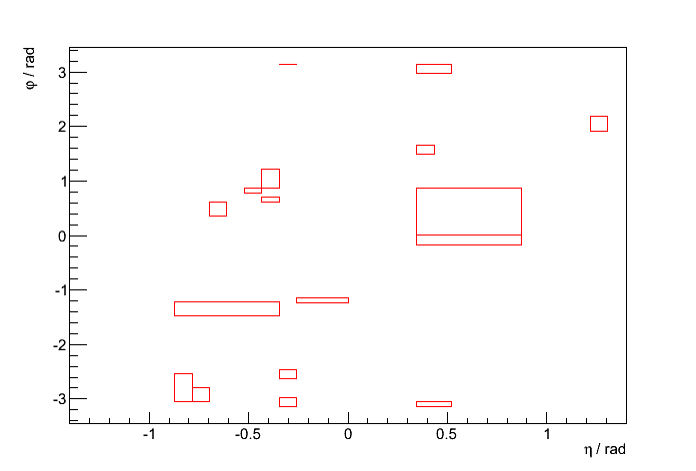
\includegraphics[width=0.45\textwidth]{Figures/erdogan/deadregions.png}
				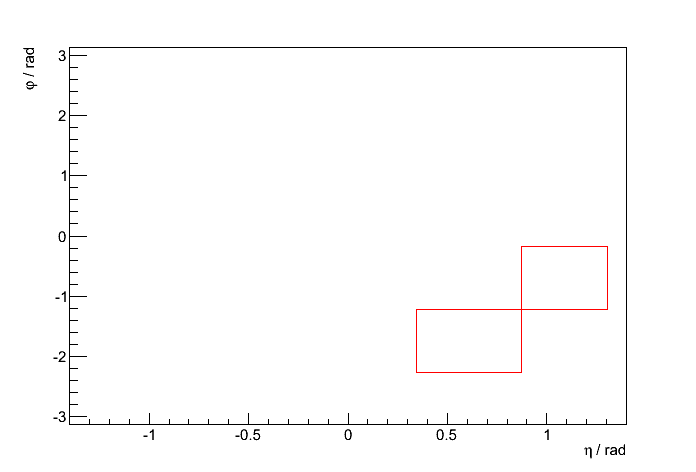
\includegraphics[width=0.45\textwidth]{Figures/erdogan/sipmregions.png}
				\caption{Left: In the $\eta-\phi$ plane, the red rectangles are showing the regions where HO is insensitive due to the supporting material or electrical issues \cite{JINST}. Right: In red
				rectangles the acceptance regions for tiles with SiPM readout (status pre LS1).}
				\label{fig:ho_acceptance}
			\end{figure}
			In figure \ref{fig:simhits_in_acceptance} the $\eta-\phi$ distribution of simulated hits of muons with $p_T = 100$\,GeV (muon gun) in HO is shown.
			\begin{figure}[htbp]
				\centering
				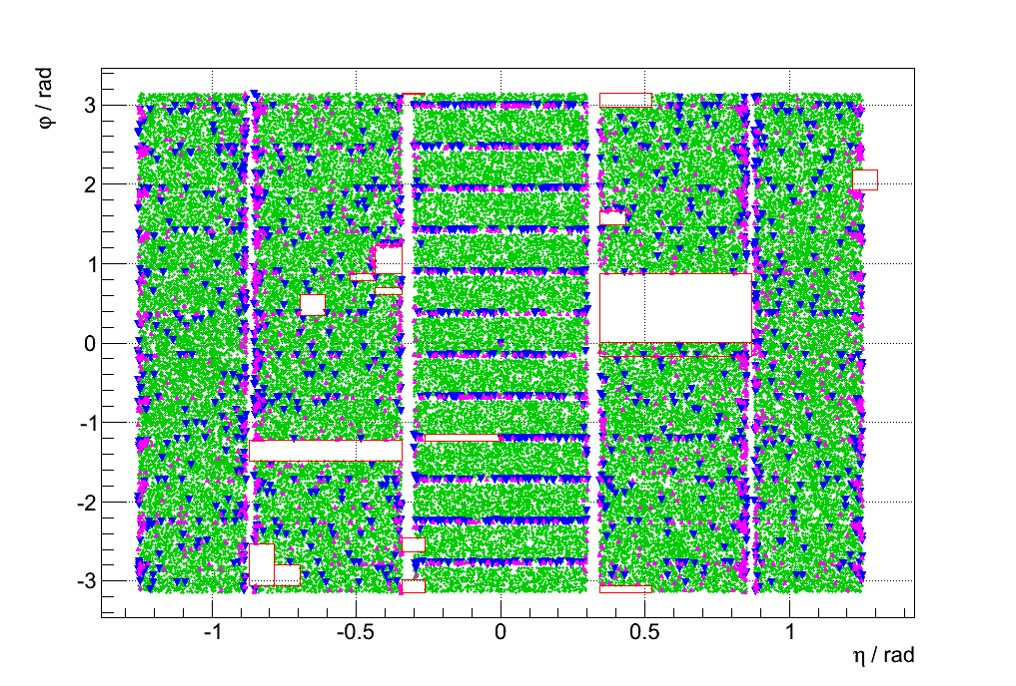
\includegraphics[width=0.45\textwidth]{Figures/erdogan/simhits_wo_deta_dphi.png}
				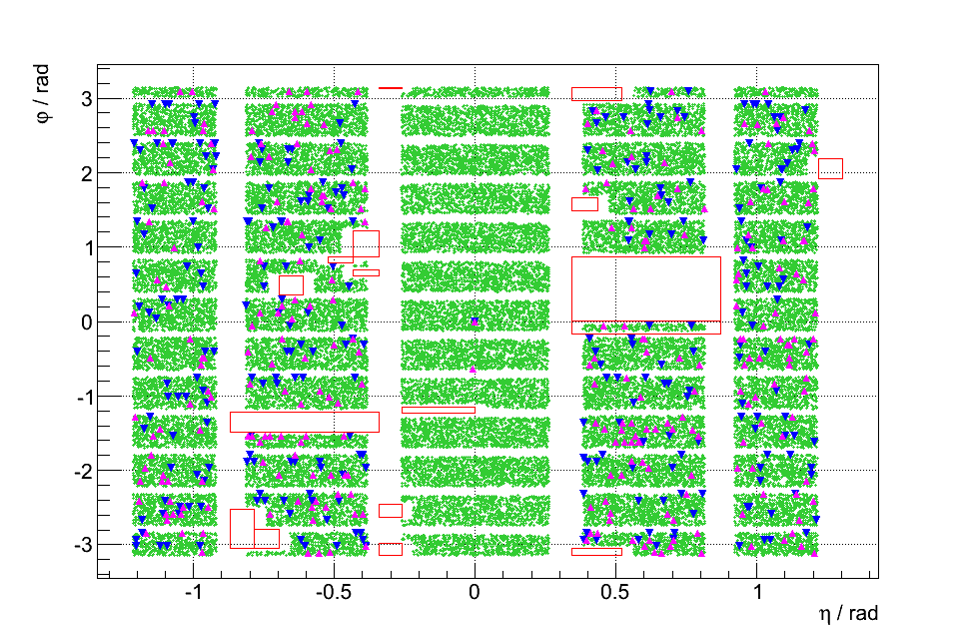
\includegraphics[width=0.45\textwidth]{Figures/erdogan/simhits_with_deta_dphi.png}
				\caption{Left: $\eta-\phi$ distribution of simulated hits of muons with $p_T = 100$\,GeV (muon gun). In green, hits from geometrically accepted muons with energy depositions above 1.4\,MeV, in
				blue, same for muons with energy depositions between 0 and 1.4\,GeV and in magenta, for muons with no energy deposition at all. The threshold at 1.4\,MeV is motivated by the Bethe-Bloch formula,
				which predicts an energy deposition of larger than 1.4\,MeV for muons going through 1\,cm scintillator material. Right: The same distribution with the safety distances $d\eta = 0.04$\,rad and
				$d\phi = 0.017$\,rad from the edges of the HO panels.}
				\label{fig:simhits_in_acceptance}
			\end{figure}
			According to this figure a large fraction of the accepted muons deposit energies predicted by the Bethe-Bloch formula.
			However there are muons going through HO tiles but depositing very low energies or no energy at all.
			These muons are located particularly at the edges of the HO panels.
			Having only scratched the HO tiles, the transition is obviously enough for very low depositions.
			Therefore it is helpful to reject those muons by defining safety margins $\Delta\eta$ and $\Delta\phi$ at the edges of the panels as it is shown on the right hand side in figure
			\ref{fig:simhits_in_acceptance}.
			By having these safety margins there is only a very small fraction of muons depositing low energies.
			These muons are uniformly distributed in $\eta-\phi$ due to the insensitive areas between the tiles.
			Furthermore in one of the geometrical rejection regions in wheel +1 ($0.3<\eta<0.9$ and $-0.2<\phi<0$) one can see hits from muons.
			Since this seems to be an error in the geometry record of the HO applied at the beginning of the events, muons in this region are not considered for the following analyses.
			Finally the safety margins in this study are chosen to be $\Delta\eta = 0.04$\,rad and $\Delta\phi = 0.017$\,rad.
			With all these considerations 1.016.286 events with exactly one muon could be selected for the study.
			In \ref{CutFlow} the cutflow can be seen.
			Thereby in each case the remaining number of events after cut is shown.
			\begin{center}
			\label{CutFlow}
				\begin{tabular}{|c|c|}
					\hline
					\textbf{cut}  & \textbf{events} \\ \hline \hline
			 		no/initial    & 13.766.979 		\\ \hline
			 		back. removal & 13.766.882 		\\ \hline
			 		prim. vertex  &  8.188.753 		\\ \hline
			 		$\eta$-$p_t$  &  8.188.753 		\\ \hline
			 		one muon      &  4.174.334 		\\ \hline
			 		tight id      &  3.820.149 		\\ \hline
			 		isolation     &  1.574.816 		\\ \hline
			 		geom. accept. &  1.016.286 		\\ \hline
				\end{tabular}
			\end{center}
			 %Obviously there are only a few events from beam background.
			 %The first cut with a big impact is the primary vertex filter.
			 %With this filter $\approx 40$\% of all events were rejected.
			 %By choosing only those events containing exactly one muon we lose approximately the half of the statistic.
			 %The next cut with a big effect is than the isolation criterion.
		\subsubsection{Matching of the muons to the corresponding HO tiles}
			Being selected as described in \ref{thesectionhere} the muons now schould be matched to the correct HO tiles.
			This is done by using the standard tracking tool \textit{TrackDetMatchInfo}.
			Doing a helix approximation this tool collects the information along a track.
			Among this information also HO related parts like the detector IDs of the tiles crossed by the muon, the reconstructed hits in these tiles or the global position of the track at HO etc. can be
			found.
			If one of the HOIDs crossed by a muon is the same as one of the IDs of a reconstructed hit in the HO system, than this muon is considered as matched.
			Since no additional requirements on the reconstructed hits - e.g. a certain energy predicted by the Bethe Bloch formula - are done, this procedure is very loose.
			Nevertheless it illustrates a best case scenario for the detection efficiency of muons in HO in 2012 data taking.
		\subsubsection{Detection efficiency for prompt muons}
			Since the HO system was read out partially by SiPMs and HPDs (see section \ref{HOIntro}), the muons flying in the tiles with SiPM readout were seperated from the muons with with HPD readout to see
			the impact of the upgrade to the SiPM readout.
			Even with the loose procedure of matching muons to the correct tiles only 393.900 muons out of 1.222.503 could be matched to the HO tiles with HPD readout.
			This leads to an efficiency of $\approx32\,\%$.
			The reason of this very low efficiency is given especially by the noise behaviour of the HPDs as decribed in \ref{HOIntro}.
			Looking into the SiPM tiles only, one expect a higher efficiency due to the better S/N ratio of the SiPMs compared to the HPDs.
			In this case out of selected 84.382 muons 72.720 muons can be matched.
			This is an efficiency of $86\,\%$.
			Although this efficiency seems to be relatively high, the expected value for a real case with realistic matching criteria should be lower.
			This is also reasonable since there is a known problem with the slow control of the first generation SiPMs used for the readout HO tiles during 2012 data taking.
			Nevertheless the improvement compared to the HPDs is clearly seen.
	\subsection{Studies on detection efficiency of cosmic muons using the GRIN data} 
		In November 2013 for one week CMS has taken data of cosmic muons during a global run (GRIN = \textbf{G}lobal \textbf{R}un \textbf{I}n \textbf{N}ovember).
		For this operation the magnet was switched off.
		The aim was to check the functionality of subsystems after the long operation break due to the first long shutdown.
		However the data can also be used to study the response behaviour of different upgraded subsystems, like HO.
		\subsubsection{Detector setup and preperation of the data}
			During the GRIN the HO system was partially used and the following parts were instrumented with the next generation SiPMs:
			\begin{itemize}
				\item All YB-2, YB-1,
				\item 7 of 12 sectors in YB0 (1, 4, 5, 7, 8, 9, 12),
				\item 2 of 12 sectors in YB+1 (3, 4),
				\item 2 of 12 sectors in YB+2 (3, 4)
			\end{itemize}
			These SiPMs have a better functionality compared to the first generation SiPMs used during the first run.
			Since the cosmic trigger was given by the moun system in the wheels YB+1, YB+2 and YB0 only the data from the corresponding parts of HO can be analyzed.
			Additionally only a few runs are marked as good for HCal/HO.
			These are 216232, 216311, 216312, 216420, 216423 and 216450.
			Having considered that, the RAW data of muons has to be reconstructed according to the standard cosmic reconstruction procedure of CMS.
			In this note we do not describe in detail the reconstruction of the hits in the HO system, since the study in this section is concentrated on the DIGI information of HO.
		\subsubsection{HO DIGI information}
			The CMS data format DIGI contains the information of the detector response to a physical process like a muon transition.
			In case of HO the measured signal is stored as counts of an analog-to-digital-converter (adc) for 10 timeslices in a HO DIGI.
			Each timeslice takes 25\,ns.
			For the calibration of the HO DIGIs it is possible to use several records registered during the data taking, like the HCalPedestalRecord or HCalElectronicsRecord.
			An alternative calibration can be done using text files filled with calibration values determined by hand.
			For this study such a calibration is done setting all pedestal corrections to 0, all gain corrections to 1 and all slope corrections to 1.
			This ensures the studied signal to be unbiased by the calibration itself, since for such short run periods like GRIN the calibration by records are not so expressive.
			In figure \ref{fig:adc_vs_ts} the calibrated adc counts versus the timeslices in which they are measured are shown.
			\begin{figure}[htbp]
				\centering
				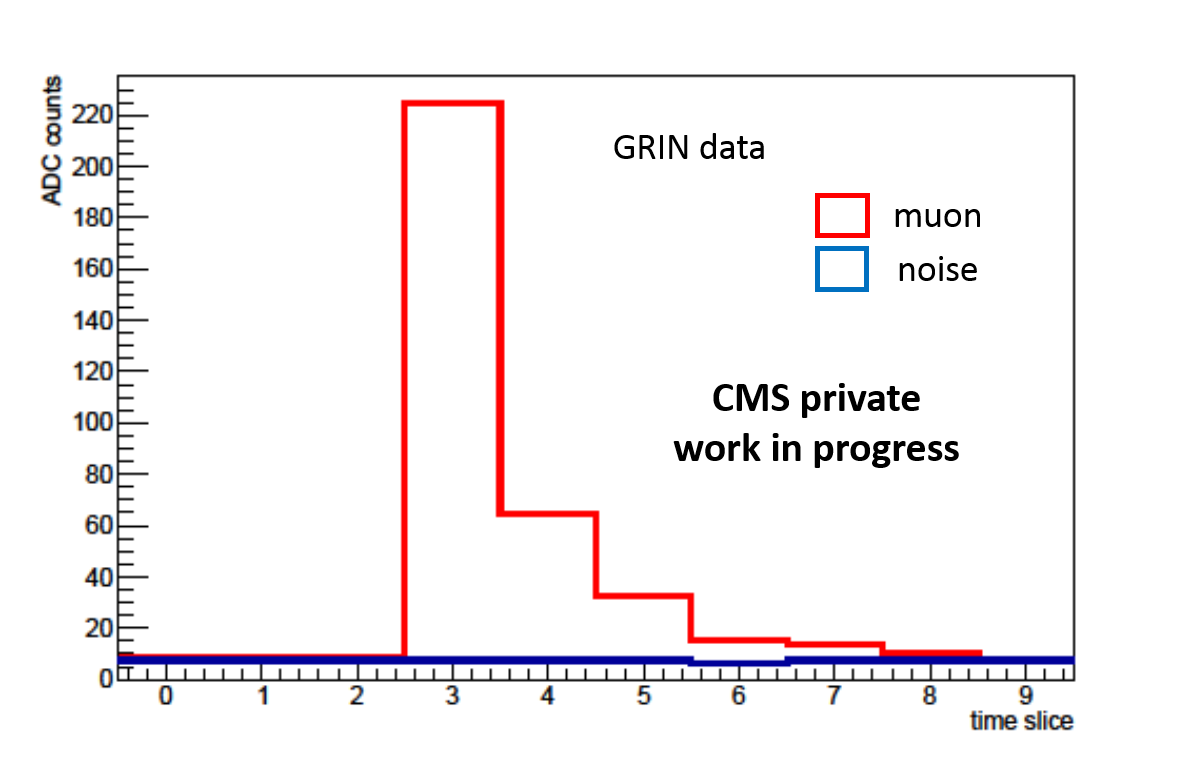
\includegraphics[width=0.45\textwidth]{Figures/erdogan/adc_vs_ts.png}
				\caption{The calibrated adc counts versus the timeslices in which they are measured: In blue a tile is chosen, where no muon is gone through (noise). In red is a tile with muon transition shown.}
				\label{fig:adc_vs_ts}
			\end{figure}
			In case of a muon transition the measured adc counts in the corresponding timeslice are clearly higher than without muon transition.
			This means distinguishing muon signal from noise should be possible.
		\subsubsection{Purity studies}
			In section \ref{sipmChapter} the funtionality of SiPMs is discussed.
			Concerning the HO data from GRIN a so-called finger spectrum can be studied.
			Therefore the signal in one randomly chosen HO tile is considered.
			In figure \ref{fig:noise_low} this signal distribution as a function of adc counts is shown for the tile XY.
			\begin{figure}[htbp]
				\centering
				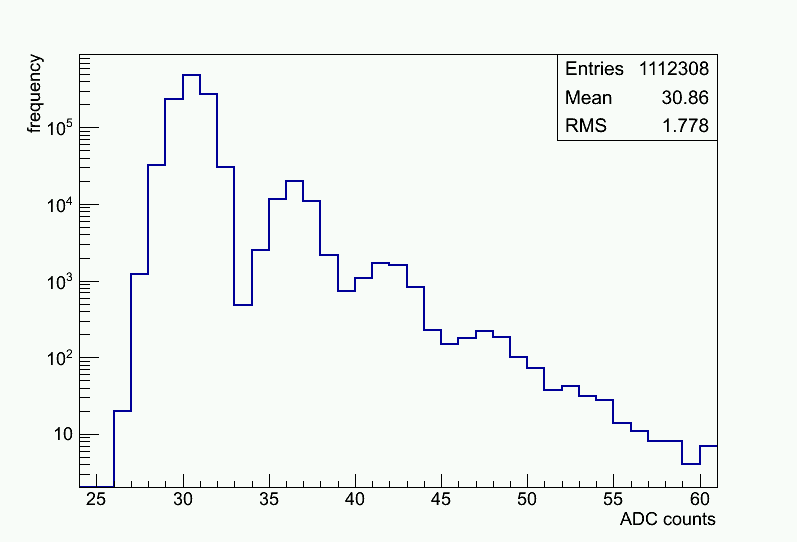
\includegraphics[width=0.45\textwidth]{Figures/erdogan/noise_low.png}
				\caption{The signal distribution as a function of adc counts for the tile XY.}
				\label{fig:noise_low}
			\end{figure}
			The first peak is the pedestal of the signal being at 36 adc counts.
			Furthermore there are 3 additional peaks corresponding to the up to 3 firing pixels of the SiPM.
			The distance between the peaks, which is the gain of the SiPM, is at 6 adc counts.
			All these observations are consistent with the expectations from the HO detector performance group (REF to ANDREAS).
			Since this study is done with only one tile per event the statistic is relatively low.
			To get more statistic and study the behaviour of the noise distribution with this higher statistic, all tiles per event without a muon transition should be taken into account.
			To do this first of all the tile where the muon went through has to be traced.
			This is done by the TrackDetMatchInfo tool described in the previous subsection.
			Afterwards a safety region of 3x3 tiles around this traced tile is defined.
			Now with all remaining tiles in all events the noise distribution can be considered (figure \ref{fig:noise_high}).
			\begin{figure}[htbp]
				\centering
				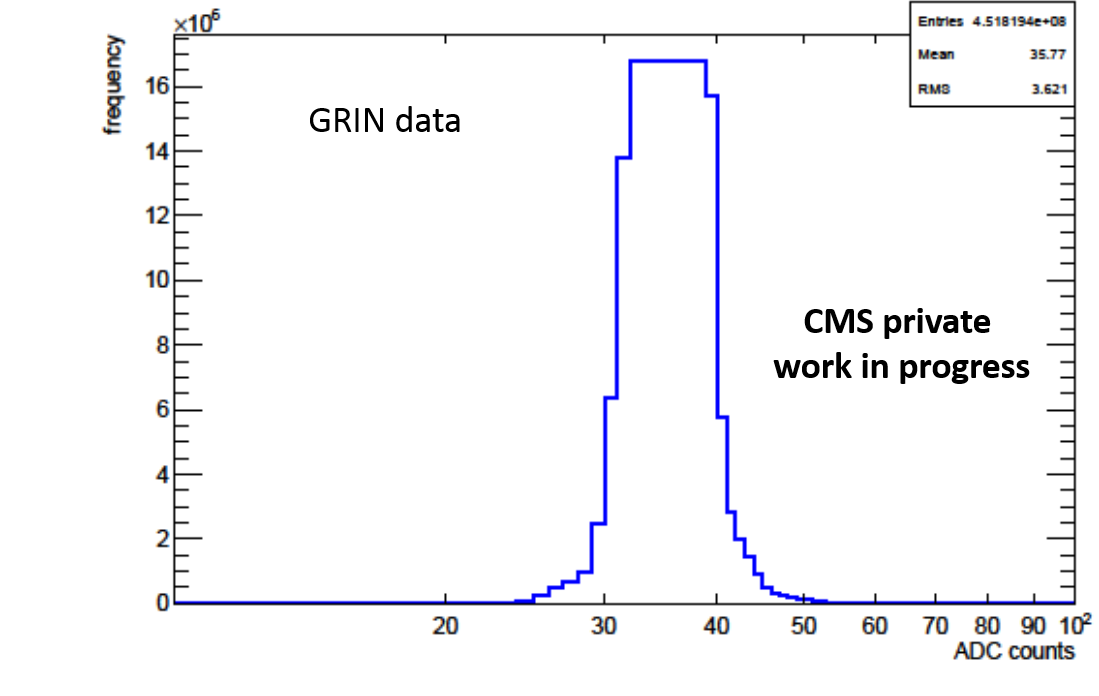
\includegraphics[width=0.45\textwidth]{Figures/erdogan/noise_high.png}
				\caption{The signal distribution as a function of adc counts for all tiles without muon transition.}
				\label{fig:noise_high}
			\end{figure}
			The mean is at 36 adc counts as expected and seen as pedestal in the distribution with low statistics.
			However the fingers are not visible anymore.
			The reason for this is the smearing of the finger due to their statistical uncertainty.
			Furthermore the distribution drops steaply until in the higher bins there is no significant contribution anymore.
			It is therefore above 80 adc counts not expected to have a noise contribution in the signal.
			With this a purity of the muon signal can be defined.
			In the section \ref{working_point} the value of 80 adc counts can be improved comparing the efficiency and the purity.
		\subsubsection{Efficiency studies}
			After having a method to estimate the purity the muon signal itself has to be analyzed.
			Using the TrackDetMatchInfo tool one can find the tiles where the muons are going through.
			Once the correct tiles are traced, the DIGI information can be looked into.
			For this purpose an integration over four timeslices is done to define the signal.
			The choice of the correct four timeslices is important and is done as described following:
			\begin{itemize}
			  \item Find the timeslice $i$ with the highest adc counts.
			  \item If $i$ between 1. and 7. timeslice (inclusively) add adc counts of the timeslice $i-1$, $i+1$ and $i+2$ to the adc counts of $i$.
			  \item If $i=0$, $i=8$ or $i=9$ take timeslices 2,3,4 and 5 for the integration.
			\end{itemize}
			In figure (\ref{fig:efficiency1x1}) the integrated value of adc counts from tiles where a muon went through is plotted.
			\begin{figure}[htbp]
				\centering
				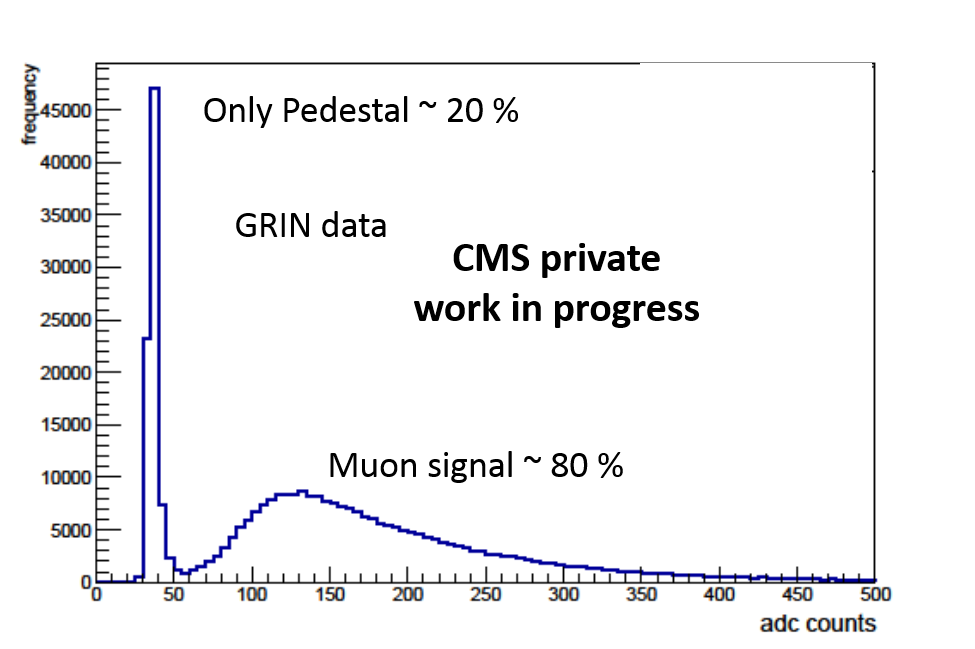
\includegraphics[width=0.45\textwidth]{Figures/erdogan/efficiency1x1.png}
				\caption{}
				\label{fig:efficiency1x1}
			\end{figure}
			Thereby the main issue is the existence of tiles with very low signals (first accumulation).
			Setting a threshold on the x axis, one can define an efficiency $e$
			\begin{equation}
				e = \frac{\textnormal{number of entries above threshold}}{\textnormal{number of all entries}},
			\end{equation}
			and the inefficiency $1-e$ respectively.
			If we set the threshold to 60 adc counts, only 80 \% of muons have a signal above threshold.
			The reason for this behaviour could be the first hint of detector inefficiencies.
			But also the functionality of the TrackDetMatchInfo tool can be doubted.
			To study the latter the search for the correct tile is not restricted to one tile predicted by TrackDetMatchInfo but all neighbor tiles of it.
			In this neighborhood the integration of timeslices is done as described above.
			The tile is chosen to be the correct tile if the value of the integrated adc counts is maximum.
			In case of the matching tool being working correctly, the search in the neighbor tiles shouldn't have an effect on the signal distribution from figure \ref{fig:efficiency1x1}.
			\begin{figure}[htbp]
				\centering
				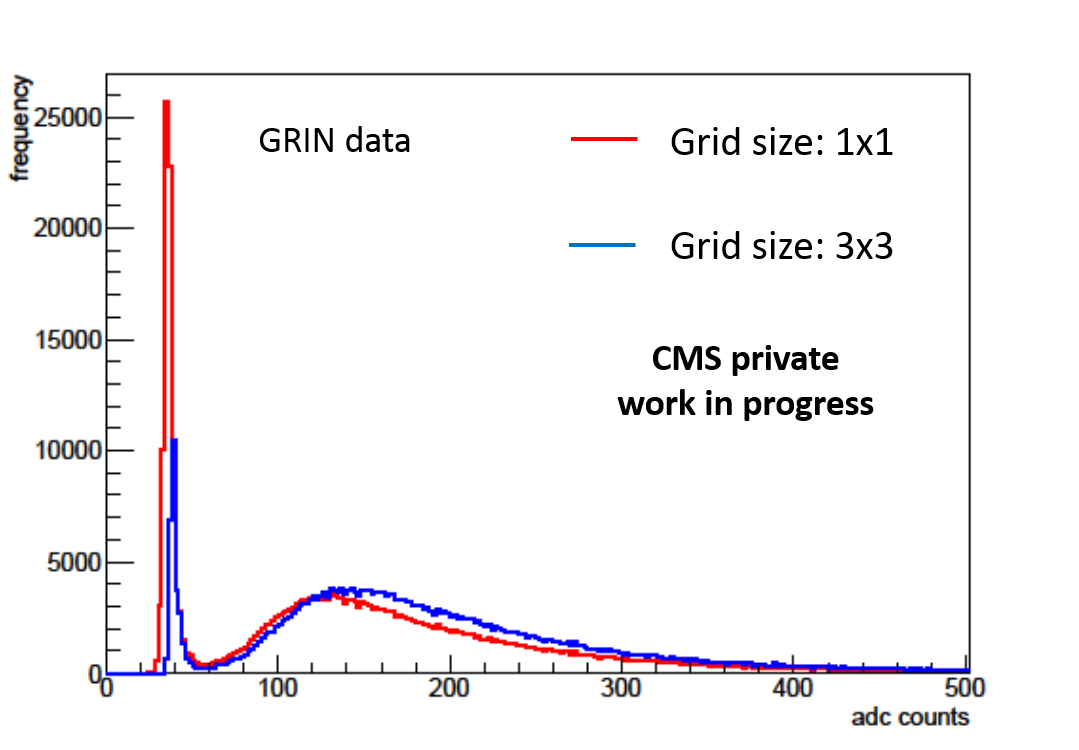
\includegraphics[width=0.45\textwidth]{Figures/erdogan/neighborhood.png}
				\caption{}
				\label{fig:neighborhood}
			\end{figure}
			But in figure \ref{fig:neighborhood} one can see the improvement of the efficiency to 92\% choosing a search area of 3x3 around the predicted tile.
			Furthermore increasing the size of this area to 7x7 has no significant effect on the distribution or efficiency.
			This means that the TrackDetMatchInfo is finding in 80\% of all cases the correct tile and in 12\% of all cases it misses the correct tile by one neighbor tile.
			The second issue is the shape of the signal.
			A gaus convoluted Landau fit on the signal (above threshold) is shown in figure \ref{fig:langaus_bad}.
			\begin{figure}[htbp]
				\centering
				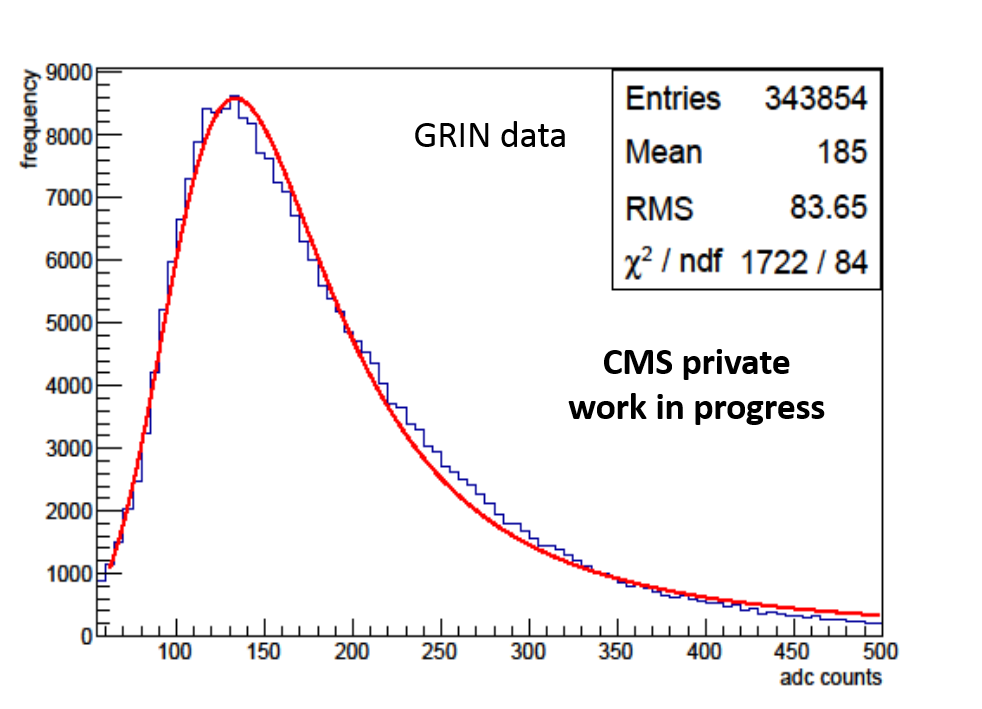
\includegraphics[width=0.45\textwidth]{Figures/erdogan/langaus_bad.png}
				\caption{}
				\label{fig:langaus_bad}
			\end{figure}
			Obviously the shape can not be described with this fit.
			The reason is the difference in distances of tiles from the readout modules.
			The intensity of the signals namely drops with the length of the fibre leading it to the readout modules.
			Therefore one has to compare only tiles with same fiber lengths.
			This is done in figure \ref{fig:langaus_good} resulting in a much better fit.
			\begin{figure}[htbp]
				\centering
				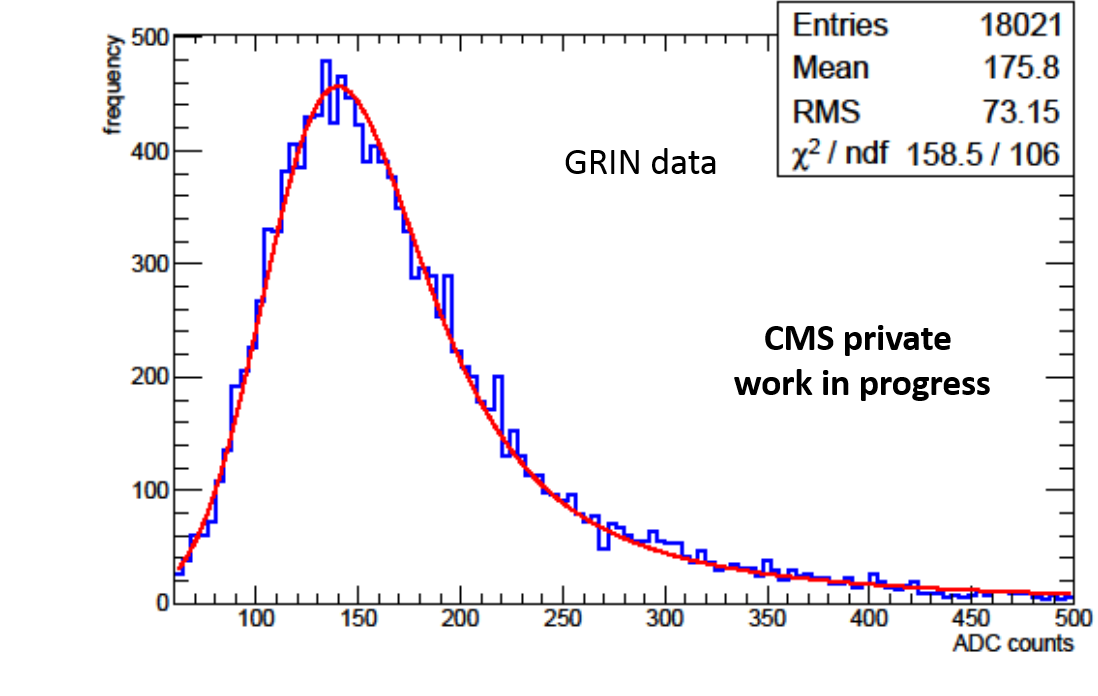
\includegraphics[width=0.45\textwidth]{Figures/erdogan/langaus_good.png}
				\caption{}
				\label{fig:langaus_good}
			\end{figure}
		\subsubsection{Working point for triggering muons}
		\label{working_point}
			The requirement to a good particle detector is especially working with high efficiency at high purity.
			In the previous sections we chose the thresholds for purity and efficiency arbitrarily by eye.
			After plotting those observables as a function of the threshold in adc counts in the same histogram, we can define a more suitable threshold.
			In figure \ref{fig:pur_eff} this histogram is depicted.
			\begin{figure}[htbp]
				\centering
				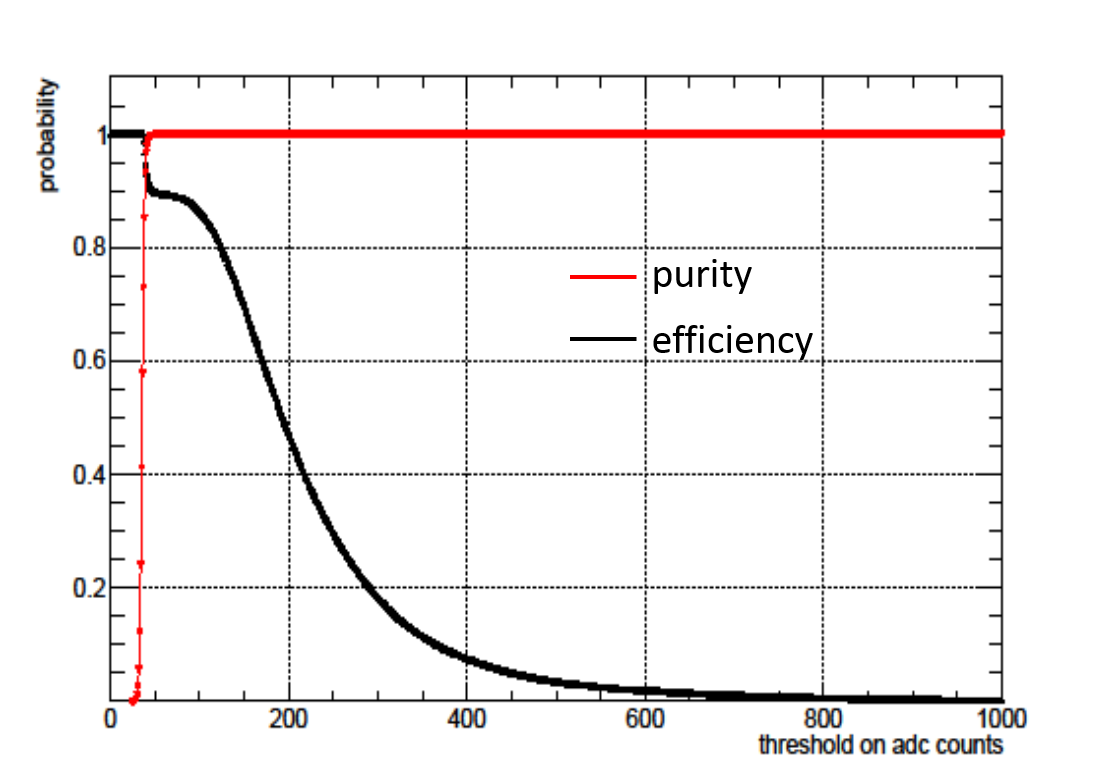
\includegraphics[width=0.45\textwidth]{Figures/erdogan/pur_eff.png}
				\caption{}
				\label{fig:pur_eff}
			\end{figure}
			The intersection point of both curves is at 39 adc counts.
			At this point the purity accounts to 95\% and the efficiency to 95\%.
			In a more concervative way one can increase the threshold to 46 adc counts leading to a highly pure signal of above 98\% by decreasing the efficiency to 90\%.